% This is samplepaper.tex, a sample chapter demonstrating the
% LLNCS macro package for Springer Computer Science proceedings;
% Version 2.20 of 2017/10/04
%
\documentclass[runningheads]{llncs}
%
%\let\proof\relax
%\let\endproof\relax
\usepackage{graphicx}
\usepackage{todonotes}
\usepackage{amsmath}
%\usepackage{amsthm}
\usepackage{braket}
% Used for displaying a sample figure. If possible, figure files should
% be included in EPS format.
%
% If you use the hyperref package, please uncomment the following line
% to display URLs in blue roman font according to Springer's eBook style:
% \renewcommand\UrlFont{\color{blue}\rmfamily}

\begin{document}
%
\title{Assessing Solution Quality of 3SAT\\on a Quantum Annealing Platform}
%
%\titlerunning{Abbreviated paper title}
% If the paper title is too long for the running head, you can set
% an abbreviated paper title here
%
\author{Thomas Gabor\inst{1} \and
Sebastian Zielinski\inst{1} \and
Sebastian Feld\inst{1} \and
Christoph Roch\inst{1} \and
Christian Seidel\inst{2} \and
Florian Neukart\inst{3} \and
Isabella Galter\inst{2} \and\\
Wolfgang Mauerer\inst{4} \and
Claudia Linnhoff-Popien\inst{1}}
%
\authorrunning{Gabor et al.}
% First names are abbreviated in the running head.
% If there are more than two authors, 'et al.' is used.
%
\institute{LMU Munich\and
Volkswagen Data:Lab \and
Volkswagen Group of America\and
OTH Regensburg/Siemens Corporate Research}
%
\maketitle              % typeset the header of the contribution
%
\begin{abstract}
When solving propositional logic satisfiability (specifically 3SAT) using quantum annealing, we analyze the effect the difficulty of different instances of the problem has on the quality of the answer returned by the quantum annealer. A high-quality response from the annealer in this case is defined by a high percentage of correct solutions among the returned answers. We show that the phase transition regarding the computational complexity of the problem, which is well-known to occur for 3SAT on classical machines (where it causes a detrimental increase in runtime), persists in some form (but possibly to a lesser extent) for quantum annealing.

\keywords{Quantum Computing \and Quantum Annealing \and D-Wave \and 3SAT \and Boolean satisfiability \and NP \and phase transition.}
\end{abstract}
%
%
%
\section{Introduction}
%Following the great paper \cite{feld2018hybrid} we thought, let's do another one!
%\todo{0.5 Introduction}

The benefit of the technology of quantum computing is essentially connected to the quantum speedup. Or rather, more generally, if quantum computing is to succeed, it needs to be faster or better or cheaper than classical computing hardware at at least one useful task.

Research in that area has cast an eye on the complexity class NP: It contains problems that are traditionally (and at the current state of knowledge regarding the P vs. NP problem) conjectured to produce instances too hard for classical computers to solve within practical time constraints. However, the problems in NP are also known to be quite susceptible to the benefits of parallelization.

As quantum mechanics has an interpretation suggesting infinite parallelism of possibilities contained within a superposition, we may have a match here. For a rather concrete implementation of quantum mechanics we focus on the technological platform of quantum annealing. Quantum annealers specialize in solving optimization problems only. As a trade-off they can as of now work rather large amounts of qubits in a useful way and are one of the few technological platforms in the area of quantum technology that are easily available to the general public.

In this paper we want to evaluate the performance of quantum annealing (or more specifically a D-Wave 2000Q machine) on the canonical problem of the class NP, i.e., propositional logic satisfiability for 3-literal clauses (3SAT) \cite{cook1971complexity}. As we note that there is still a remarkable gap between 3SAT instances that can be put on a current D-Wave chip and 3SAT instances that even remotely pose a challenge to classical solvers, there is little sense in comparing the quantum annealing method to classical algorithms in this case. Instead, we are most interested in the scaling behavior with respect to problem difficulty. Or more precisely: We analyze if and to what extent quantum annealing's performance suffers under hard problem instances (like classical algorithms do).

To this end, we present a quick run-down of 3SAT and the phenomenon of phase transitions in Section~\ref{sec:preliminaries} and continue to discuss further related work in Section~\ref{sec:related-work}. In Section~\ref{sec:exp-setup} we describe our experimental setup and then present the corresponding results in Section~\ref{sec:evaluation}. We conclude with Section~\ref{sec:conclusion}.

\section{Preliminaries}
\label{sec:preliminaries}
\todo{1 SAT w/ Phase Transition}


\subsection{Phase transitions in SAT solving}
Diese Phasenübergangsgrenze teilt den Problemraum in zwei Regionen. In der einen Region kann eine Lösung relativ leicht gefunden werden, da die Lösungsdichte für diese Probleme hoch ist, in der anderen Region ist es sehr unwahrscheinlich, dass Probleme überhaupt eine korrekte Lösung enthalten können. Sehr schwer zu lösende Probleme befinden sich direkt an der Phasenübergangsgrenze \cite{cheeseman1991really}. Bei den in dieser Arbeit betrachteten 3SAT-Problemen liegt diese Phasenübergangsgrenze bei einem Klausel zu Variablenverhältnis von ca. 4.267~\cite{mezard2002random}.

TODO: See Figure~\ref{fig:distr}.
\begin{figure}
\centering
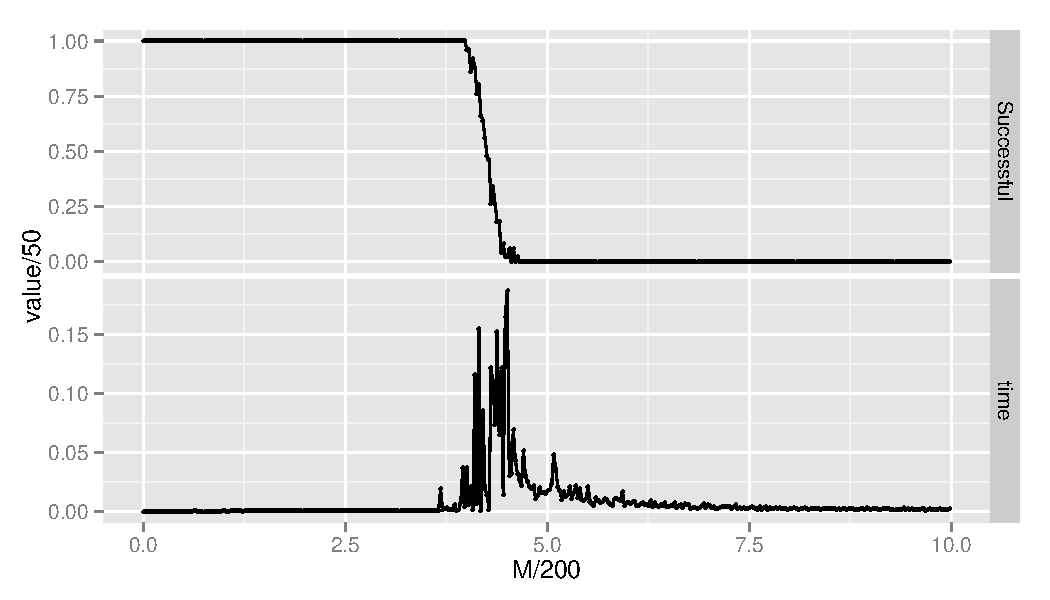
\includegraphics[width=.8\textwidth]{../material_2/plot_sat.pdf}
\caption{Loesungsfindungsdauer von 3SAT-Instanzen mit 1000 Klauseln für ver- schiedene Anzahl von Variablen.} \label{fig:distr}
\end{figure}

Das K -Erfüllbarkeitsproblem (im Folgenden\emph{ KSAT} genannt) gehört zur Klasse der NP-Vollständigen Probleme. KSAT ist, für K > 3, ein zentrales Problem in der kombinatorischen Optimierung und war das erste Problem, für das die NP-Vollständigkeit gezeigt werden konnte \cite{mezard2002random}.

Problembeschreibung: K - Erfüllbarkeitsproblem (nach  \cite{mezard2002random})
Gegeben sei eine Menge $\mathcal{B}$, bestehend aus N booleschen Variablen. Aus dieser Menge $\mathcal{B}$ werden dann K Variablen ausgewählt. Die ausgewählten Variablen, oder deren Verneinungen, werden dann durch (K-1) Oder-Operatoren zu einer \emph {Klausel} zusammengefasst. Auf diese Art und Weise werden M Klauseln gebildet. Durch anwenden von (M-1) Und - Operatoren entsteht so eine KSAT-Instanz.\\Das KSAT-Problem ist nun die Frage, ob eine Belegung der boolschen Variablen aus $\mathcal{B}$ existiert, so dass eine gegebene KSAT-Instanz erfüllbar ist.

In dieser Arbeit werden ausschließlich zufällig generierte KSAT-Instanzen für K=3 betrachtet. Diese Probleme werden dann 3SAT genannt und sind nach \cite{cook1971complexity} NP-Vollständing.

\subsection{Kritischer Punkt bei zufällig generierten KSAT-Instanzen}\label{krit:sat}
Bei zufällig generierten KSAT-Instanen kann beobachtet werden, die Wahrscheinlichkeit, eine korrekte Lösung für die Instanz zu finden, abrupt sinkt, wenn ein kritischer Wert $\alpha_{c}$ (gebildet aus dem Verhältnis von Anzahl der Klauseln zu Anzahl der Variablen) überschritten wird \cite{monasson1996entropy}.

Nach \cite{mezard2002random} liegt dieser kritische Punkt bei zufällig erzeugten 3SAT-Instanzen bei \\$\alpha_{c} \approx 4,267$. In der Umgebung des kritschen Punkts ist die Lösungsfindung (damit ist hier nicht nur eine konkrete Belegung gemeint, falls die Instanz lösbar ist, sondern auch die Erkenntnis, dass diese Instanz nicht gelöst werden kann) algorithmisch komplex. Abb. \ref{crit_sat} verdeutlicht dieses Phänomen visuell.

Zur Erstellung von Abb. \ref{crit_sat} wurden mit Hilfe des \emph{Tough SAT Generators}\footnote{https://toughsat.appspot.com/} 3SAT-Instanzen zu je 1000 Klauseln erstellt. Die Größe der  Menge der boolschen Variablen wurde ausgehend von 1000 schrittweise um 10 verringert, bis ein abschließendes Klausel zu Variablenverhältnis von ca. 7 erreicht wurde. Für jede Größe der so erzeugten Variablenmenge wurden 10 Instanzen erzeugt. Die verschiedenen Instanzen wurden dann mit dem SAT-Solver \emph{Minisat}\footnote{http://minisat.se/} gelöst. In Abb. \ref{crit_sat} ist dann einmal die durchschnittliche sowie die maximale Lösungsdauer der 10 Instanzen für ein bestimmtes Verhältnis dargestellt.
 %%%%%%%%%%%%%%%%% Maximum-Weight Independetn Set %%%%%%%%%%%%%%%%%%%%%%%%%%%%%%%%%%%%%%%%%%%%
%\subsection{Das Problem der maximal gewichteten unabhängigen Menge}\label{chap:wmis}
%
%--Unabhängige Menge \cite{feo1994greedy}]\label{def:unabhmenge}
%Gegeben sei ein Graph $\mathcal{G} = (V,E)$, wobei V die Menge der Knoten des Graphs ist und E die Menge der Kanten des Graphs.\\Eine \emph{unabhängige Menge} von $\mathcal{G}$ ist eine Menge V' $\subset$ V mit folgender Eigenschaft:
%\begin{equation}
%(i,j) \notin E \;\;\;\forall i,j \in V' 
%\end{equation}
%Eine \emph{unabhänginge Menge} eines Graphen $\mathcal{G}$ ist also eine Teilmenge V' der Knoten von $\mathcal{G}$ so, dass die Knoten aus V' paarweise nicht direkt durch eine Kante von $\mathcal{G}$  verbunden sind.
%
%--Maximal gewichtete unabhängige Menge \cite{choi2010adiabatic}
%Gegeben sei ein ungerichteter Graph $\mathcal{G} = (V, E)$, wobei V die Menge der Knoten und E die Menge der Kanten von $\mathcal{G}$ sind, bei dem jeder Knoten v $\in$ V mit einem positiven reellen Gewicht $c_{v}$ versehen wird.\\
%Das Problem ist es dann eine Menge S $\subset$ V zu finden, so dass S eine unabhängige Menge im Sinne von Def. \ref{def:unabhmenge} ist und das Gesamtgewicht von S, gegeben durch $\sum_{v \in S} c_{v}$, maximal ist. Die optimale Lösung wird auch mit WMIS($\mathcal{G}$ ) bezeichnet.
%
%\noindent
%Das Problem der maximal gewichteten unabhängingen Menge wird im Folgenden \emph{WMIS} (engl. Weighted Maximum Independent Set) genannt. Für dieses Problem existiert die folgende QUBO-Darstellung:
%
%Es sei der gleiche Graph $\mathcal{G}$ wie aus der vorhergehenden Problembeschreibung gegeben. Die QUBO-Formulierung des WMIS-Problems lautet dann:
%\begin{equation}\label{wmis:qubo}
%Maximiere \;\;\mathcal{Y}(x_{1},...,x_{n}) = \sum_{i \in V}c_{i}x_{i} - \sum_{i,j \in E}J_{ij}x_{i}x_{j}
%\end{equation}
%
%
%Ist in gerade definierter QUBO-Darstellung des WMIS-Problems $J_{ij} > min \{c_{i},c_{j}\}$ für alle i,j $\in$ E dann ist das WMIS von $\mathcal{G}$ gegeben durch $WMIS(\mathcal{G})=\{v \in V: x^*_{v}=1\}$, wobei $(x^*_{1},...,x^*_{n})$ = arg $max_{(x_{1},...x_{n})\in{0,1}^n} \mathcal{Y}(x_{1},...,x_{n}).$
%
%Es sei  $(x^*_{1},...,x^*_{n})$ = arg $max_{(x_{1},...x_{n})\in{0,1}^n} \mathcal{Y}(x_{1},...,x_{n})$. Weiter sei S* = $\{v \in V: x^*_{v}=1\}$ gegeben. Angenommen, S* ist keine unabhängige Menge. Es gibt also zwei Knoten x,y $\in$ S* die durch eine Kante aus $\mathcal{G}$ verbunden sind. Ohne Beschränkung der Allgemeinheit kann angenommen werden, dass $c_{x} < c_{y}$ gilt. Als nächstes entfernt man x aus S* und bezeichnet mit S' = S*\textbackslash\{x\} die so entstandene Menge. Das Gewicht von S' unterscheidet sich dann durch das Gewicht von S* durch den Ausdruck $-c_{x} + \sum_{j \in nbr(y) \cap S^*}J_{ij} > -c_{y} + J_{yz} > 0$, mit nbr(y) = $\{ z \in V: (z,y) \in E\}$. Das bedeutet also S' hat ein größeres Gewicht als S*, was einen Widerspruch zur Optimalität von S* darstellt. Die Annahme muss also falsch gewesen sein und S* muss eine unabhängige Menge sein. 

\section{Related Work}
\label{sec:related-work}

It is one of the cornerstones of complexity theory that solving NP-complete or even NP-hard decision problems is strongly believed to be not efficiently possible~\cite{cook1971complexity,murty1987some}. Any NP-complete problem can also be cast as an optimization problem, which allows for employing well-known optimization algorithms to find approximate solutions---typical methods include tabu search \cite{glover2013tabu,gendreau1994tabu} and simulated annealing \cite{kirkpatrick1983optimization,chen1995chaotic}. Countless other efficient approximation methods, together with an elaborate taxonomy on approximation quality (how much does a given solution differ from a known global optimum?) and computational effort (how many time steps are required until an approximate solution that satisfies given quality goals is available?), have been devised \cite{Ausiello1999}.

Some problem (knapsack, e.g.) exhibit favorable properties when cast as an optimization problem. The latter is a member of the complexity class FPTAS (fully polynomial-time approximation scheme), which means that a solution with distance \(1+\epsilon\) (of course, $\epsilon > 0$) from an optimal solution can be determined in polynomial time in both, input size \(n\) and inverse approximation quality \(1/\epsilon\)~\cite{chen1995chaotic}.

An intriguing connection that has received substantial attraction exists between (computational) NP-complete problems and the (physical) concept of phase transitions, as detailed in Section~\ref{sec:preliminaries}. First investigations of the phenomenon have been performed by Kirkpatrick et al.~\cite{kirkpatrick1994critical}; Monasson et al.\ first suggested a connection between the type of phase transition and the associated computational costs of a problem~\cite{monasson1999determining}. From the abundant amount of more recent investigations, we would like to highlight the proof by Ding et al.~\cite{ding2015proof} that establishes a threshold value for the phase transition. Our work benefits from the above insights by selecting the ``most interesting'', i.e., computationally hardest, scenarios as investigation target.

The idea of obtaining solutions for NPO (NP optimization) problems by finding the energy ground state (or states) of a quantum mechanical system was used, for instance, by Apolloni et al.~\cite{apolloni1989quantum,apolloni1988numerical} to solve combinatorial optimization problems. The general idea of quantum annealing has been independently re-discovered multiple times~\cite{albash2016adiabatic,finnila1994quantum,amara1993global,kadowaki1998quantum}.

Quantum annealing techniques are usually applied to solving NP-complete or NP-hard decision problems, or optimization problems from class NPO. Lucas~\cite{lucas2014ising} reviews how to formulate a set of key NP problems in the language of adiabatic quantum computing respectively quadratic unconstrained binary optimization (QUBO). In particular, problems of the types ``travelling salesman'' or ``binary satisfiability'' that are expected to have a major impact on practical computational applications if they can be solved advantageously on quantum annealers have undergone a considerable amount of research~\cite{heim2017designing,warren2017small,moylett2017quantum,strand2017zzz,benjamin2017measurement,neukart2017traffic}. Further effort has been made on combining classical and quantum methods on these problems~\cite{feld2018hybrid}.

Comparing the computational capabilities of classical and quantum computers is an intriguing and complex task, since the deployed resources are typically very dissimilar. For instance, the amount of instructions required to execute a particular algorithm is one of the main measures of efficiency or practicability on a classical machine, whereas the notion of a discrete computational ``step'' is hard to define on a quantum annealing device. Interest in quantum computing has also spawned definitions of new complexity classes (e.g., \cite{klauck2017complexity,morimae2017merlinization}), whose relations to traditional complexity classes have been and are still subject to ongoing research~\cite{bernstein1997quantum,marriott2005quantum}.

% TODO: Hier brauchen wir in der endgueltigen Version auf jeden Fall
% noch bessere Referenzen.

These questions hold regardless of any specific physical or conceptual implementation of quantum computing since their overall computational capabilities are known to be largely interchangeable; for instance, McGeoch~\cite{mcgeoch2014adiabatic} discusses the
equivalence of gate-based and adiabatic quantum computing. Consequently,
our work focuses not on comparing quantum and classical aspects of solving particular problems, but concentrates on understanding peculiarities
of solving one particular problem (3SAT, in our case) in-depth.

Formulating 3SAT problems on a quantum annealing hardware has been previously considered~\cite{choi2011different,choi2010adiabatic,farhi2000quantum}, and we rely on the encoding techniques presented there. Van~\cite{van2001powerful} and Farhi~\cite{farhi2009quantum} have worked on analyzing the complexity of solving general 3SAT problems. Hsu et al. have considered the complexity-wise easier variation 2SAT for benchmarking quantum annealers~\cite{hsu2018quantum}.
 

\section{Experimental Setup}
\label{sec:exp-setup}

Quantum annealing is an optimization process that can be implemented in hardware. It is built upon the adiabatic theorem that provides conditions under which an initial ground-state configuration of a system evolves to the ground state of another configuration that minimizes a specific user-defined energy function~\cite{mcgeoch2014adiabatic}. As in the real world the required conditions for the theorem can only be approximated, the results of quantum annealing are usually not exact but show a probabilistic distribution, ideally covering the desired optimal value as well.

D-Wave's quantum annealer is the first commercial machine to implement quantum annealing. Its interface is built on two equivalent mathematical models for optimization problems called Ising and QUBO, the latter of which will be used for the work of this paper. Quadratic Unconstrained Binary Optimization (QUBO) problems can be formulated as a quadratic matrix $Q_{ij}$. Quantum annealing then searches for a vector $x \in \{0,1\}^n$ so that $\sum_i \sum_{j < i} Q_{ij} x_i x_j + \sum_i Q_i x_i$ is minimal. The promise of quantum annealing is that---using quantum effects---specialized hardware architectures are able to solve these optimization problems much faster than classical computers in the future.

The main goal of this paper is to analyze the inherently probabilistic distribution of return values generated by quantum annealing when trying to solve hard optimization problems. We choose to demonstrate such an analysis on 3SAT because it is the canonical problem of the class NP, which is a prime target for research on performance improvements via quantum technology with respect to classical computers~\cite{mcgeoch2013experimental,lucas2014ising}.

\subsection{Defining 3SAT as a QUBO}
3SAT is usually not formulated as an optimization problem (see Section~\ref{sec:preliminaries}), or defined by an equivalent QUBO problem,
as is required by the annealer. Thus, we require a (polynomial-time) translation of any 3SAT instance into a QUBO so that the solutions generated by the quantum annealer can be translated back to solutions of the initial 3SAT instance.

Following~\cite{choi2010adiabatic,choi2011different}, we translate 3SAT into the Weak Maximum Independent Set (WMIS) problem (which we covered in Section~\ref{sec:preliminaries}), and then translate the WMIS instance into a QUBO (we find it convenient to specify the polynomial coefficients in matrix form). We omit the details of the process and instead refer to \emph{op.~cit.{}} and Ref.~\cite{lucas2014ising}. However, we shall briefly discuss the implications of the translation process.

A 3SAT instance, that is, a formula with $m$ clauses for $n$ variables,
requires a QUBO matrix of size $3m \times 3m$ with the solution vector $x \in \{0,1\}^{3m}$. The solution can be thought of as using a qubit for each literal in the initial formula and thus consisting of a triplet of qubits for each 3SAT clause. This usually means that we have much more qubits than variables in the formula. Nonetheless, a QUBO solution is mapped to a value assignment for the variables in the 3SAT formula. Thus, when running successfully, the quantum annealer will output a satisfying assignment for a given 3SAT formula. We can check if the assignment really is correct (i.e., each variable has a value assigned and the whole formula reduces to $\textit{True}$) using few instructions of classical computation. Obviously, if among several experimental runs the quantum annealer does return just one correct assignment, the corresponding 3SAT formula is satisfiable. If the quantum annealer only returns incorrect assignments, we will regard the formula as unsatisfiable (although the prove of that is only probabilistic).

There are some aspects to note about how the QUBO solution vectors are mapped to variable assignments. Given a QUBO solution vector $(x_i)_{0 \leq i \leq 3m-1}$ for a 3SAT formula with literals $(l_i)_{0 \leq i \leq 3m-1}$, a variable $v$ is assigned the value $\textit{True}$ if it occurs in a literal $l_i = v$ and $x_i = 1$. Likewise, a variable $v$ is assigned the value $\textit{False}$ if it occurs in a literal $l_i = \lnot v$ and $x_i = 1$. It is important to note that $x_i = 0$ has \emph{no implication} on the value of the variable in $l_i$.

Intuitively, we can interpret $x_i = 1$ to mean ``use the value of $l_i$ to prove the satisfaction of clause $c_{(i \mod 3)}$''. From our QUBO optimization, we expect to find one (and only one) suitable $l_i$ for every clause in the 3SAT formula.\footnote{This intuition matches the concept of constructivism in logic and mathematics. We are not only looking for the correct answer, but are looking for a correct and complete proof of an answer, giving us a single argument for each part of the formula.}

This is important as it opens up a wide range of different QUBO solutions which may just encode the exact same variable assignment at the 3SAT level. However, it also means that seemingly suboptimal QUBO solutions may encode correct 3SAT assignments. For example, consider the (a little redundant) 3SAT formula $(v_0 \lor v_1 \lor v_2) \land (v_0 \lor v_1 \lor v_2)$: The QUBO solution $x = 100001$ would imply the assignment of $v_0 = \textit{True}$ and $v_2 = \textit{True}$, which indeed is theoretically sufficient to prove the formula satisfiable. The exact same assignment would be implied by $x = 001100$. However, note that none of these imply a full assignment of every variable in the 3SAT instance since none say anything about the value of $v_1$. Still, we can trivially set $v_1$ to any arbitrary value and end up with a correct assignment. Also note that while the QUBO is built in such a way to opt for one single value $1$ per triplet in the bit string, even bitstrings violating this property can encode correct solution. In our example, the suboptimal QUBO solution $x=100000$ still encodes all necessary information to prove satisfiability.

\subsection{Evaluating Postprocessing}

As can be seen from the last example, postprocessing is an integral part of solving problems with quantum annealing. As discussed earlier in this section, we consider a QUBO solution correct if it not only matches the expected structure for minimizing the QUBO energy function, but instead iff it directly implies a correct assignment in the definition given above. Thus, while the expected structure for QUBO optimizes $x$ so that the amount bits $x_i$ assigned $1$ equals the amount of clauses $m$, we also consider less full answers correct.

On top of that, there are solutions that cannot be mapped to an assignment immediately, but still with almost no effort. We want to regard these as well and implemented a postprocessing step we call \emph{logical postprocessing}. It is applied whenever none of the qubits corresponding to a single clause $c_k$ are set to $1$ by the quantum annealer and the respective QUBO solution is not already correct. In that case, we iterate through all literals $l_i$ in that clause $c_k$ and check if we could set $x_i = 1$ without contradicting any other assignment made within $x$. If we find such an $l_i$, we set $x_i = 1$ and return the altered bitstring $x$.

The software platform provided by D-Wave to use the quantum annealer already offers integrated postprocessing methods as well, which we will also empirically show to be more powerful than logical postprocessing in the following Section~\ref{sec:evaluation}. Again, for greater detail we refer to the D-Wave documentation on that matter~\cite{dwavepostprocessing}. At a glance, the employed postprocessing method splits the QUBO matrix into several subproblems, tries to optimize these locally, and then integrates that local solution into the complete solution if it yields an improvement. We call this method \emph{D-Wave postprocessing}.

To evaluate the solution quality regarding 3SAT, we employ both methods. The goal is to assess the expected quality on a 3SAT-to-3SAT level, that is, we measure how well we can solve the given 3SAT instance and regard the translation to and from QUBO as a mere technical problem that is not of
interest for this paper.

%$c_k = (l_{3k} \lor l_{3k+1} \lor l_{3k+2})$ 


%
%
%\todo{0.5 SAT via WMIS on QA}
%\todo{1 Experimental Setup}
%
%
%\subsection{Optimierungs-Postprocessing des D-Wave}
%Nachdem ein Problem via Quantumannealing gelöst wurde, stellt der D-Wave Quantenannealer zusätzlich die Möglichkeit verschiedener Arten von Postprocessing bereit. In dieser Arbeit wird ausschließlich das Optimierungs-Postprocessing des D-Wave benutzt.\\\\Das Ziel des Optimierungs-Postprocessings ist es, eine Menge an Lösungen zu erhalten, die auf einem bestimmten Graphen $\mathcal{G}$ die geringste Energie aufweisen. Um dies zu erreichen, wird ein gegebener Graph $\mathcal{G}$ durch eine heuristische Methode (vgl. \cite{markowitz1957elimination}) in mehrere Teilgraphen zerlegt. Danach wird die bereits von der QPU erhaltene Lösung so verändert, dass für jeden Subgraphen eine lokal optimale Lösung entsteht. Für eine tiefergehende Darstellung des Postprocessings auf dem D-Wave sei an dieser Stelle auf die D-Wave Dokumentation zu diesem Thema (siehe \cite{dwavepostprocessing}) verwiesen, in welcher auch der hier dargestellte grobe Überblick über das Optimierungs-Postprocessing gefunden werden kann.
%%%%%%%%%%%%% LOGISCHES POSTPROCESSING %%%%%%%%%%%%
%\subsection{Logisches Postprocessing}
%Zusätzlich zum D-Wave Optimierungs-Postprocessing wird in dieser Arbeit ein vom Autor dieser Arbeit erdachtes logisches Postprocessing verwendet, um die ursprünglichen Ergebnisse der QPU weiter zu verbessern. Bei diesem logischen Postprocessing, wird eine von der QPU erhaltene Lösung, welche ein Spinarray der Länge 3\emph{m} ist, wobei \emph{m} die Anzahl der Klauseln in einem 3SAT-Problem darstellt, zurück auf eine Variablenbelegung der logischen Variablen des 3SAT-Problems abgebildet. Danach wird überprüft ob es nicht erfüllte Klauseln gibt. Ist dies der Fall, so wird für jede Variable einer nicht erfüllten Klausel überprüft, ob deren Negation bereits die Belegung \emph{wahr} erhalten hat. Ist dies nicht der Fall, so kann der betrachteten Variable der Wahrheitswert \emph{wahr} zugewiesen werden. In diesem Fall werden weitere Variablen dieser Klausel nicht mehr angesehen und es wird direkt mit der nächsten nicht erfüllten Klausel fortgefahren.
%


\section{Evaluation}

Wie in Abschnitt \ref{krit:sat} dargelet wurde, gibt es bei 3SAT-Instanzen signifikante Unterschiede bezüglich der Schwierigkeit der Lösungsfindung. Das Verhältnis aus Anzahl der Klauseln zur Größe des Variablenpools , im Folgenden \emph{K/V-Verhältnis} genannt, bestimmt dabei die Schwierigkeit der Lösungsfindung. Unter Berücksichtigung dieses Sachverhalts werden im Folgenden zwei Versuchsreihen durchgeführt.
\subsection{2. Versuchsreihe}
In der 2. Versuchsreihe werden mit Hilfe des ToughSAT-Generators jeweils 100 zufällig generierte 3SAT-Formeln für die K/V-Verhältnisse 0.2, 4.2 sowie 8.4 erzeugt. Alle 3SAT-Formeln bestehen aus 42 Klauseln. Damit stehen zur Erzeugung der Formeln beim  K/V-Verhältnis von 0.2 insgesamt 210 Variablen, beim K/V-Verhältnis von 4.2 insgesamt 10 Variablen und beim K/V-Verhältnis von 8.4 insgesamt 5 Variablen zur Verfügung. Analog zur 1. Versuchsreihe werden hier alle 100 3SAT-Formeln der K/V-Verhältnisse 0.2 sowie 4.2 so gewählt, dass sie erfüllbar sind. Alle 3SAT-Formeln des K/V-Verhältnisses 8.4 sind so gewählt, dass sie nicht erfüllbar sind.
\subsection{Versuchsdurchführung}
Jedes 3SAT-Problem der 1. sowie der 2. Versuchsreihe wird zunächst auf ein WMIS-Problem reduziert (vgl. Kapitel \ref{red:sat:wmis}). Die Knoten des durch diese Reduktion entstanden Graphen \emph{$G_{SAT}$} werden mit dem  Gewicht 1 belegt, sämtliche Kanten mit dem Gewicht 4. Die Gewichte sind hier beliebig gewählt, jedoch so, dass das Kantengewicht jeder Kante größer ist als das Minimum der Gewichte der Knoten die diese Kante verbindet (vgl. Behauptung in Kapitel \ref{chap:wmis}). Anschließend werden aus diesem Graphen die linearen Gewichte der Ising-Energiefunktion berechnet (vgl. Gleichung \ref{red:6} bzw. \ref{red:7}). Nun kann das Problem dem DWAVE-Quantenannealer übergeben werden, der zunächst ein Embedding dieses Problems auf dem Chimera-Graphen bestimmt und anschließend durch Quantum Annealing eine Lösungs des Problems bestimmt. Für jede der in dieser Arbeit benutzten 3SAT-Formeln wird lediglich ein Embedding berechnet, welches dann für 1000 Annealingvorgänge benutzt wird. Man erhält also pro Formel insgesamt 1000 potentielle Lösungen.

\todo{1 Colourful Pictures (6.11, 6.12, 6.15, 6.19 + Numbers from Tab. 6.4)}
\todo{1 Explaining the colourful pictures}

\begin{figure}
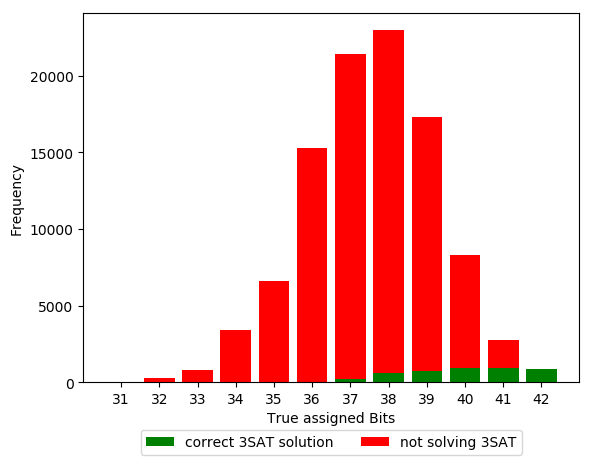
\includegraphics[width=.5\textwidth]{../material_2/Plots/42_4_2_def_engl_color_ohne_transform.png}%
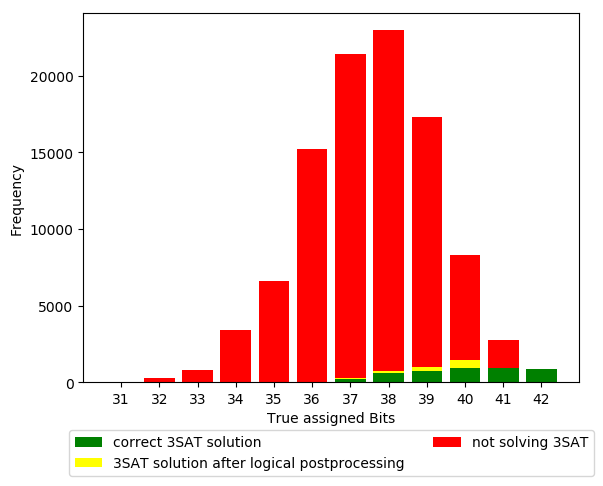
\includegraphics[width=.5\textwidth]{../material_2/Plots/42_4_2_def_engl_color_mit_transform.png}
\caption{Verteilung korrekter und nicht korrekter Antwortbitstrings ohne logisches Postprocessing (links) und mit logischem Postprocessing (rechts) für 3SAT-Instanzen bestehend aus 42 Klauseln und einem K/V- Verhältnis von 4,2.} \label{fig:distr}
\end{figure}

\begin{figure}
\centering
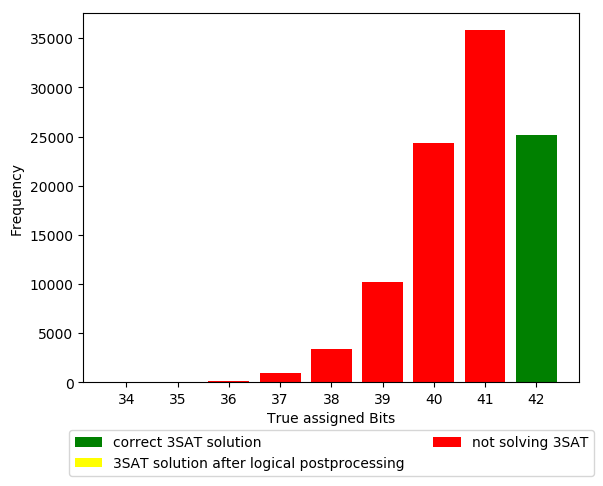
\includegraphics[width=.8\textwidth]{../material_2/Plots/42_4_2_opt_engl_color_mit_transform.png}
\caption{Verteilung korrekter und nicht korrekter Antwortbitstrings mit logischem Postprocessing für 3SAT-Instanzen bestehend aus 42 Klauseln und einem K/V- Verhältnis von 4,2.} \label{fig:distr}
\end{figure}

\begin{figure}
\centering
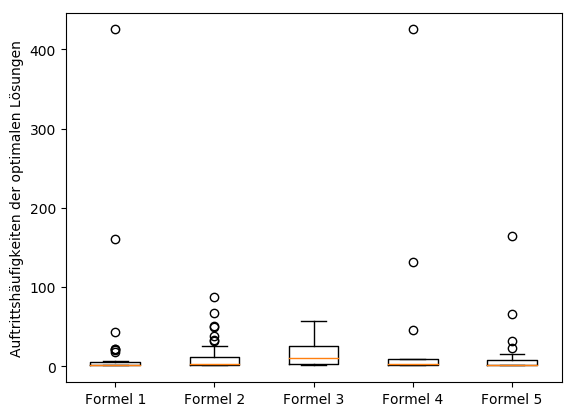
\includegraphics[width=.8\textwidth]{../material_2/25_clauses__4_2_def_MISBIAS.png}
\caption{Auftrittshäufigkeiten verschiedener optimaler Lösungen für verschiedene 3SAT-Formeln.} \label{fig:distr}
\end{figure}

\begin{figure}
\centering
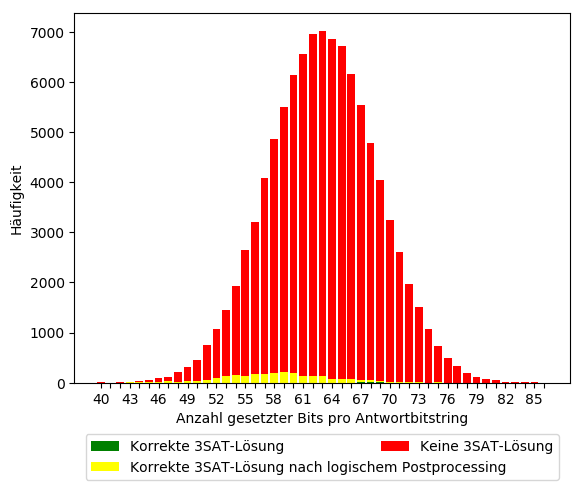
\includegraphics[width=.8\textwidth]{../material_2/42_clauses__0_2_def_RANDOM_color_transformed.png}%
%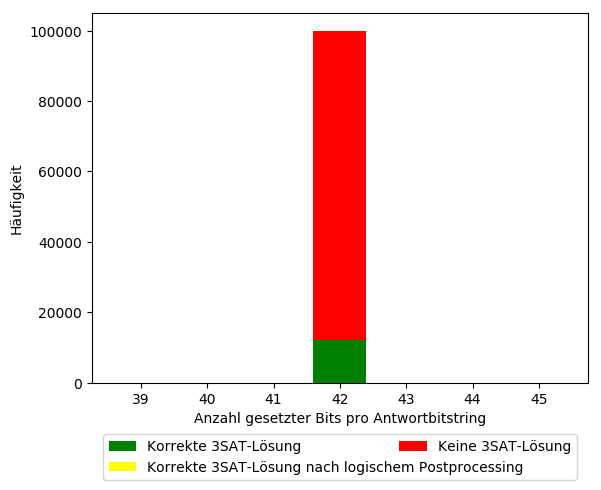
\includegraphics[width=.5\textwidth]{../material_2/42_clauses__0_2_def_RANDOM_CLEVER_color_transformed.png}
\caption{Verteilung korrekter 3SAT-Lösungen und falschen Antworten unter Ant- wortbitstrings, die durch den naiven Zufallsgenerator erzeugt wurden, mit bestimmter Anzahl gesetzter Bits für 3SAT-Formeln bestehend aus 42 Klauseln.} \label{fig:distr}
\end{figure}

\section{Conclusion}
\label{sec:conclusion}

%\todo{1 Discussion \& Conclusion (7.5.3)}

We have shown that problem difficulty of 3SAT instances also affects the performance of quantum annealing as it does for classical algorithms. However, bound by the nature of both approaches, the effects are quite different with complete classical algorithms showing longer runtimes and quantum annealing showing less precision. A first quantification of that loss of precision suggests that it may not be too detrimental and comparatively easy to deal with. However, because of to the maximum available chip size for quantum annealing hardware at the moment, no large-scale test could be performed. No real assumptions on the scaling of this phenomenon (and thus the eventual real-world benefit) can be made yet.

Our results suggest there are cases where single solutions from a set of equally optimal solutions are much more likely to be returned than others. This observation is in line with other literature on the results of quantum annealing. However, it is interesting to note that it translates into the original problem space of 3SAT.

The observed results will gain more practical relevance with larger chip sizes for quantum annealers. We thus suggest to perform these and/or similar tests for future editions of quantum annealing hardware. If the effects persist, they can indicate a substantial advantage of quantum hardware over other known approaches for solving NP-complete problems.


\section*{Acknowledgement}
Research was funded by Volkswagen Group, department Group IT. 
%
% ---- Bibliography ----
%
% BibTeX users should specify bibliography style 'splncs04'.
% References will then be sorted and formatted in the correct style.
%
\bibliographystyle{splncs04}
\bibliography{references}
%

\end{document}
